\documentclass{beamer}

\usetheme{Warsaw}
\useoutertheme {miniframes}

\usepackage{xeCJK}
\setCJKmainfont{HanWangWCL06}

\begin{document}

\title[Linkit 7688 Duo Tutorial]{Linkit 7688 Duo Tutorial}

\author{Iblis Lin}

\date{2017/6/16}

\begin{frame}
  \titlepage
\end{frame}


\section{Big Picture}

\begin{frame}{Big Picture}
  \begin{center}
    \Huge
    把溫溼度 sensor data \\
    \uncover<2->{用 Linkit 讀出後,\\}
    \uncover<4->{透過網路,\\}
    \uncover<3->{塞進資料庫,\\}
    顯示在手機上
  \end{center}
\end{frame}


\section{Env setup}

\begin{frame}{Env setup}
  \begin{itemize}
    \item code \& slide: \url{https://github.com/APCLab/ict-iot}

    \item *Windows only* \url{https://support.apple.com/kb/DL999?viewlocale=en_US&locale=en_US}
  \end{itemize}
\end{frame}

\begin{frame}[fragile]{Config Linkit}
  \Large
  \begin{itemize}
    \item 預設 Linkit 會作為一個 AP,可共連線

    \item 第一次 login 時,使用 \verb|mylinkit.local| 連線

    \item 先改密碼!
  \end{itemize}
\end{frame}

\begin{frame}[fragile]{Config Linkit Hostname}
  \Large
  \begin{center}
    改一下 hostname,避免大家用相同的
  \end{center}

  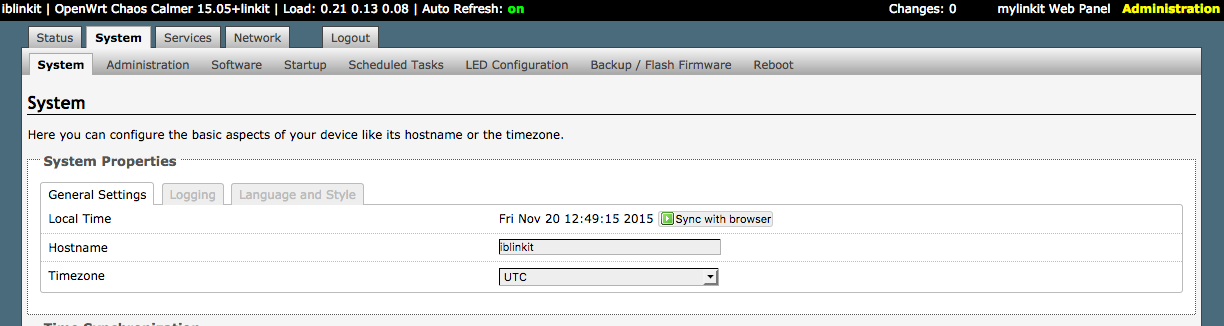
\includegraphics[scale=0.25]{./img/hostname.png}

  \begin{center}
    我的是 \verb`iblinkit`

    之後使用 \verb`iblinkit.local` 連線
  \end{center}
\end{frame}

\begin{frame}{Config Linkit Network}
  \Large
  \begin{center}
    最後回來改掉 AP mode

    換成 station mode 以連上其他 wifi AP
    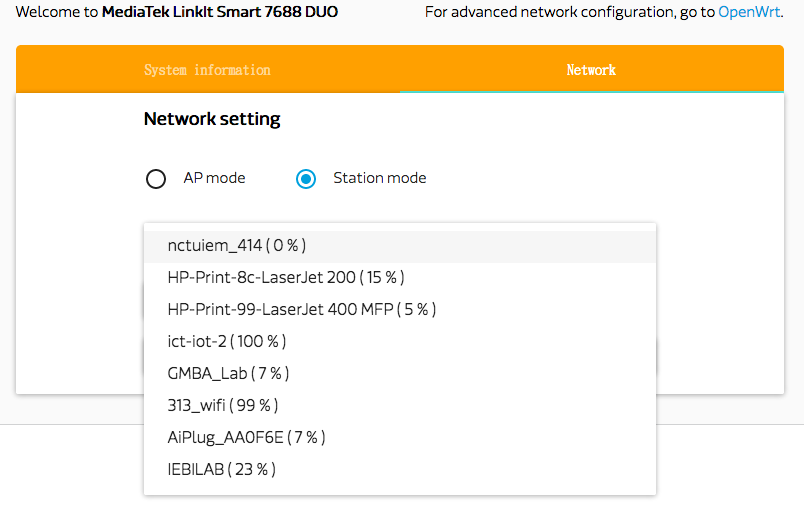
\includegraphics[scale=0.3]{./img/connect_wifi.png}
  \end{center}
\end{frame}

\begin{frame}{Config Arduino IDE}
  \Large
  Arduino 安裝 Linkit 的 Plugin

  > Perference

  \small
  \url{http://download.labs.mediatek.com/package_mtk_linkit_smart_7688_test_index.json}
\end{frame}


\section{Linkit}

\begin{frame}
  \begin{center}
    \Huge
    Linkit 讀取 sensor data

    \small
    ref:
    \url{https://goo.gl/eEHc18}
  \end{center}
\end{frame}

\begin{frame}[fragile]{Linkit Patch}
  \begin{center}
    \large
    剛好我們手上的 Linkit 裡面的軟體有 Bug

    走 ssh 連進去改 code
  \end{center}

  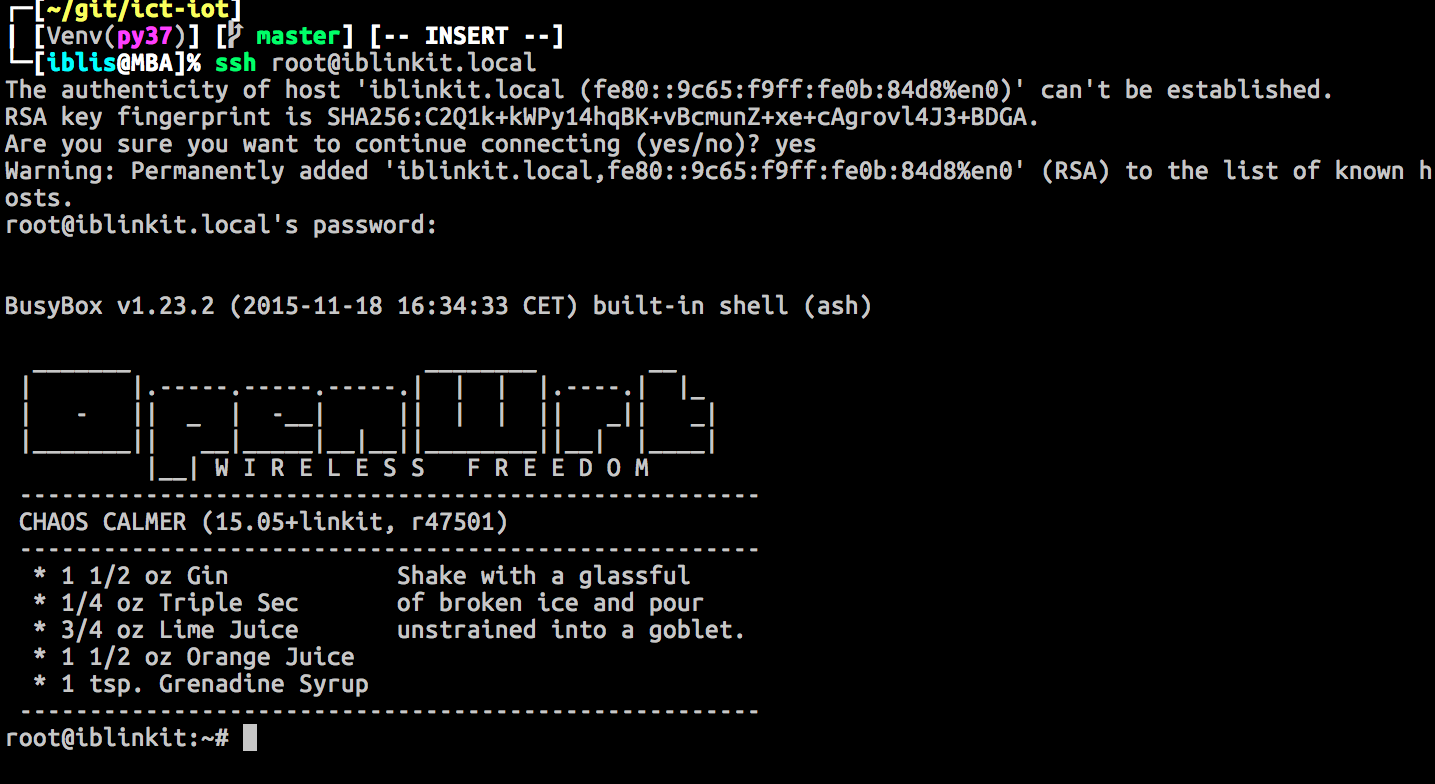
\includegraphics[scale=0.215]{./img/ssh.png}
\end{frame}

\begin{frame}{Linkit Patch}
  \Huge
  我們連上的是 Linux

  名為 OpenWrt 的 distribution
\end{frame}

\begin{frame}[fragile]{Linkit Patch}
  \tiny
  \begin{verbatim}
    vi /usr/bin/run-avrdude

    -avrdude -c linuxgpio -C /etc/avrdude.conf -p m32u4 -U flash:w:/etc/arduino/Caterina-smart7688.hex -Uflash:w:$1 $2
    +avrdude -c linuxgpio -C /etc/avrdude.conf -p m32u4 -e -v -Uflash:w:$1 $2
  \end{verbatim}

  \begin{center}
    \small
    patch: \url{https://goo.gl/xr8hpu}
  \end{center}
\end{frame}

\begin{frame}[fragile]{Linkit Config}
  \begin{center}
    \large
    打開 bridge 的功能

    MCU <--> CPU

    \begin{verbatim}
      uci set yunbridge.config.disabled='0'
      uci commit
      reboot
    \end{verbatim}
  \end{center}
\end{frame}

\begin{frame}[fragile]{Plugin sensor}
  \Large
  \begin{itemize}
    \item 這次的 溫溼度計 是 analogy sensor
    \item 型號: DHT22
    \item 接在開發板的 \verb`A0`
    \item 接電腦的 usb 選下面那個孔
  \end{itemize}
\end{frame}

\begin{frame}[fragile]{Burn code}
  \huge
  \begin{center}
    Sample code:

    \verb`linkit-7688-duo/dht22`

    reference: \url{https://goo.gl/deMXpU}
  \end{center}

\end{frame}

\begin{frame}[fragile]{Python bridge}
  \Large
  把 Python code 丟上去跑

  Sample code: \verb`linkit-7688-duo/dht22/py`

  丟上去: \verb`scp -r linkit-7688-duo/dht22/py root@iblinkit.local:~`
\end{frame}

\begin{frame}[fragile]{Python bridge}
  \begin{center}
    \Large
    \begin{verbatim}
      python py/basic.py
    \end{verbatim}
  \end{center}
\end{frame}

\begin{frame}[fragile]{Python send to DataBase}
  \Large
  我們需要額外的套件處理 Http request

  \begin{verbatim}
    pip install requests
  \end{verbatim}
\end{frame}

\begin{frame}[fragile]{Python send to DataBase}
  \Large
  \begin{itemize}
    \item 再去 \url{http://lbp.firc.tw:3000/iot/} 開個新的表格

    \item 記下我們的 id

    \item 改一下 \verb`py/to_db.py` 裡面的 id, 不要改到別人的
  \end{itemize}


  Run!
  \begin{verbatim}
    python py/to_db.py
  \end{verbatim}
\end{frame}


\section{appmate}

\begin{frame}{appmate overview}
  \Large

  \begin{itemize}
    \item 簡單的 Web application

    \item Django project

    \item 所以是使用 Python

    \item 提供 與 database 互動的 http API

    \item API 採用 REST design

    \item 我們把它設計成 template project
  \end{itemize}
\end{frame}

\begin{frame}[fragile]{appmate setup}

  建立 database, 這裡預設是使用 SQLite
  \begin{block}{code}
  \begin{verbatim}
    python ./maange.py migrate
  \end{verbatim}
  \end{block}

  建立 Django 後臺的 admin user
  \begin{block}{code}
  \begin{verbatim}
    python ./manage.py createsuperuser
  \end{verbatim}
  \end{block}
\end{frame}

\begin{frame}[fragile]{appmate setup}
  Run the server!
  \begin{block}{code}
  \begin{verbatim}
    python ./manage.py runserver
  \end{verbatim}
  \end{block}

  並且仔細看看畫面上的訊息
\end{frame}

\begin{frame}{appmate}
  \begin{itemize}
    \item check \url{http://lbp.firc.tw:3000/}

    \item check \url{http://lbp.firc.tw:3000/iot/}
  \end{itemize}
\end{frame}

\end{document}
